\documentclass{article}
\usepackage{tikz}
\usetikzlibrary{arrows.meta,positioning,calc,shapes.geometric}
\pagestyle{empty}
\begin{document}
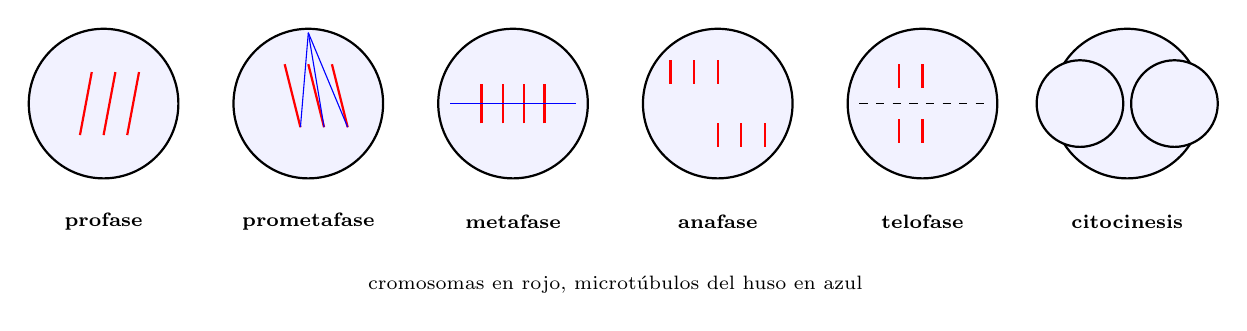
\begin{tikzpicture}

\def\cellf#1#2{\draw[thick, fill=blue!5] (#1,0) circle (0.95); \node[font=\bfseries\scriptsize] at (#1,-1.5) {#2};}
\cellf{0}{profase}\cellf{2.6}{prometafase}\cellf{5.2}{metafase}\cellf{7.8}{anafase}\cellf{10.4}{telofase}\cellf{13.0}{citocinesis}
\foreach \x in {-0.3,0,0.3} {\draw[thick, red] (\x,-0.4) -- (\x+0.15,0.4);}
\foreach \x in {2.5,2.8,3.1} {\draw[thick, red] (\x,-0.3) -- (\x-0.2,0.5); \draw[blue] (\x,-0.3) -- (2.6,0.9);}
\foreach \x in {-0.4,-0.13,0.14,0.4} {\draw[thick, red] (5.2+\x,-0.25) -- (5.2+\x,0.25);} \draw[blue] (4.4,0) -- (6.0,0);
\foreach \x in {-0.3,0,0.3} {\draw[thick, red] (7.8+\x-0.3,0.55) -- (7.8+\x-0.3,0.25); \draw[thick, red] (7.8+\x+0.3,-0.55) -- (7.8+\x+0.3,-0.25);}
\draw[thick, red] (10.1,0.5) -- (10.1,0.2); \draw[thick, red] (10.4,0.5) -- (10.4,0.2); \draw[thick, red] (10.1,-0.5) -- (10.1,-0.2); \draw[thick, red] (10.4,-0.5) -- (10.4,-0.2); \draw[dashed] (9.6,0) -- (11.2,0);
\draw[thick, fill=blue!5] (12.4,0) circle (0.55); \draw[thick, fill=blue!5] (13.6,0) circle (0.55);
\node[font=\scriptsize, align=center] at (6.5,-2.3) {cromosomas en rojo, microtúbulos del huso en azul};

\end{tikzpicture}
\end{document}
